\section{Objective}

We want to build a framework hidden for the developer that he could run on any RTOS with any application. This framework would be present between the kernel space (the RTOS) and the user space (the application) and acts as a middleware as represented by the figure \ref{fig:bench-framework-layers}.

\begin{figure}[!ht]
  \centering
  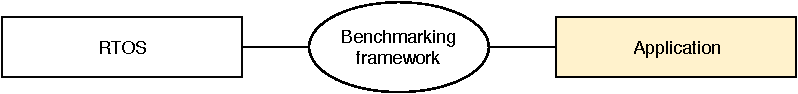
\includegraphics[scale=1]{assets/bench-framework-layers.pdf}
  \caption{\label{fig:bench-framework-layers}Internal benchmarking framework layers}
\end{figure}

The motivation for this framework is to have a system easy to use and completely hidden for the developer.
By using as little configuration as needed, the developer would have access to usefull information for developping its application.
The framework would be able to retrieve measurements such as the context switching time, the interrupt latency, the memory usage or the energy consumption.
Such measurements are commonly retrieved using an oscilloscope.
However, that kind of hardware is costly and not everyone can have access to such device.

An ideal use case for our benchmarking framework is explained in the section below.
This scenario is hypothetic and does not represent the state of our work.

\subsection{Use case}
Ideally, using our benchmarking framework, the use case for any developer using a RTOS would be the following.

The developer develops an application with multiple tasks on a specific RTOS on a specific device.
The developer wants to measure the performance of its application and, to do so, set a flag in the Makefile of its application to turn on the benchmarking framework.
The developer flashes its application on the device and the framework output continuously benchmarking information.
The information contains context switching time, interrupt latency, memory usage and enery consumption.

With this framework, the developer can optimize its application, change the device or even the RTOS.
The framework, available on as much RTOS as possible, will help the developer to see which RTOS or devices is the best fit for its application.

\subsection{Simple task}
We implemented a simple application under Contiki.
The application contains two indentical tasks.
The tasks wait for 1ms in the foreground and then goes to the background letting the scheduler runs the next task.
The tasks run in an infinite loop.
The source code of the tasks are shown in the listing \ref{lst:simple-task-code}.

\begin{lstlisting}[style=CStyle, label={lst:simple-task-code}, caption={Source code of the simple task implemented in Contiki}]
PROCESS_THREAD(task, ev, data)
{
    PROCESS_BEGIN();

    while (1)
    {
        PROCESS_PAUSE();
        // Wait for 1ms
        clock_delay_usec(1000);
    }

    PROCESS_END();
}
\end{lstlisting}


We choose to use Contiki for this measurement for its cooperative scheduling.
This kind of scheduling allows us to know when a task is in the foreground and when it goes to the background.
With a preemptive scheduling, in the other hand, we don't know when the task is preempted.
This issue is discussed later in our work.